\documentclass{report}
\usepackage[utf8]{inputenc}
\usepackage{authblk}
\usepackage{caption}
\usepackage{xcolor}
\usepackage{subcaption}
\usepackage{cite}
\usepackage{float}
\usepackage{booktabs}
\usepackage{biblatex}
\addbibresource{me353.bib}
\usepackage{graphicx}
\usepackage{hyperref}
\hypersetup{
    colorlinks=true,
    linkcolor=blue,
    filecolor=magenta,      
    urlcolor=cyan,
}

\newcommand\todo[1]{\textcolor{red}{#1}}
\renewcommand\thesection{\arabic{section}}

\title{\bfseries{Automated Warehouse Management System \\ \large{ME353 Project Report}}}

\author[1]{Drishika Nadella}
\author[2]{Kriti Shukla}

\affil[1]{181ME222, Department of Mechanical Engineering, NITK}
\affil[2]{181ME239, Department of Mechanical Engineering, NITK}

\date{29th March 2021}

\begin{document}

\maketitle

\tableofcontents
\listoffigures

\section{Introduction}

A warehouse is a building used to store goods. The goods can be provided by the manufacturer for storage, which will be shipped to the customers from the warehouse. The stored goods can be raw materials, finished products, parts, packing materials in a plethora of domains such as agriculture, telecommunications, sports, semiconductors etc.

Warehouse management is the control and optimization of warehouse activities, right from the entry of a product into the warehouse until it is moved or sold. It involves several operations such as loading and unloading, packaging, storing, retrieval, picking, inspection etc.

Warehouse management is often confused with inventory management, but they are not the same. While inventory management deals with the actual goods or the inventory themselves, warehouse management is the overall management of all warehouse operations to ensure the optimal storage of the inventory.

There are several private companies in India that provide warehouse storage facility for a range of manufacturers. The All India Warehousing Pvt Ltd (AIW) is one such warehousing company. The functioning of the company can be seen in \href{https://www.youtube.com/watch?v=cAQ3jQVAniA}{this video}.

AIW is a private warehousing company in Mumbai that has about 350,000 sq ft of warehousing space. It stores many different types of goods, ranging from industrial, food to pharmaceuticals. The goods can be raw or finished. The warehouse quality system is in accordance with ISO 9001 2015. There are four locations in Mumbai, all strategically placed such that they are in close vicinity to major highways, the railway network as well as the ports.

The AIW warehouses have several features, as seen in the video:

\begin{itemize}
    \item {\bfseries Storage and Retrieval System:} As seen in the video, the storage and retrieval of goods is done manually, or through human operated forklifts. The various storage boxes are placed rather unsystematically on the floor or simple racks.
    \item {\bfseries Order Picking:} The order picking is done by the warehouse workers manually or through machines such as forklifts.
    \item {\bfseries Order Packaging and Inspection:} The order packaging and inspection is done by the warehouse workers manually.
    \item {\bfseries Temperature Control:} AIW stores some perishable goods and temperature sensitive pharmaceuticals, which require rigorous temperature control.
    \item {\bfseries Seasonal or Cyclical Inventory:} Some of the products stored in the AIW warehouses are replenished seasonally or periodically.
    \item {\bfseries Security System:} AIW has several security measures to ensure the safety of the stored goods, such as CCTV systems, Automatic Card Access and Door locking systems.
    \item {\bfseries Fire System:} The warehouse has sprinkler systems and automatic fire hydrants.
    \item {\bfseries Warehouse Management System:} AIW has its order information in paper records that are stored in the warehouse as well as a software database management system.
\end{itemize}

\section{Motivation}

Currently, the AIW warehouses are predominantly handled by humans, such as product loading and unloading, or human operated machines, such as forklifts. The storage of the various components is not systematic, which can result in inventory mismanagement. Such a warehouse system is prone to inefficiency, errors caused by humans, more effort and less reliability. 

There are several advantages of automating a warehouse system:

\begin{itemize}
    \item {\bfseries It saves time:} Automating warehouse functions such as inventory management, product storage and retrieval, packaging etc saves manual time.
    \item {\bfseries It is efficient:} When we automate inventory storage, picking, retrieval, loading, unloading etc, it is performed efficiently by automated systems that work in a streamlined and orderly manner.
    \item {\bfseries It is accurate:} It becomes very difficult to keep track of hundreds of products in the inventory, as well as their movement through the warehouse manually. Hence, automated systems provide better accuracy.
\end{itemize}

All these factors reduce cost, time and human labour significantly and contribute to the long-term success of the warehouse. In addition, automated warehouses are also energy saving, safe and can function unattended \cite{Deng2018DevelopmentOA}. 

Since automation has not yet been adopted well by AIW, our motivation with this project is to suggest some automation techniques to their warehouse in order to increase their efficiency. We believe this would be especially useful to the company since, during COVID-19, sales through e-commerce and online deliveries have sky-rocketed. Therefore, it is important to automate warehouse operations to improve the efficiency and keep up with the demand.

\section{Problem Statement}

The problem statement we have chosen is to improve the working of All India Warehousing Pvt Ltd by introducing automated systems in several domains of warehouse management, thereby improving their productivity and effectiveness.

\section{Research Methodology}

Due to travel restrictions and safety concerns due to COVID-19, we could not visit a physical industry to assess the functioning of the industry, and to determine how to better incorporate automation into the operations.

Therefore, we decided to assess an industry in the next best way: by searching for a virtual tour of industries on YouTube. We looked for industries that were known to be established, and where the videos provided a well-rounded tour of the facility. 

We chose All India Warehousing Pvt Ltd because:

\begin{itemize}
    \item It is a registered private company that is listed on the internet.
    \item The video provided information regarding the company in a well-rounded manner, similar to having visited the facility itself.
    \item There was major scope for automation to be introduced to the industry since many of the operations were performed by humans, or by human operated machines.
    \item There is a lot of reference technical material on the internet regarding warehouse automation, and it is an important industry, especially so during COVID-19, where online e-commerce deliveries have seen a major demand. 
\end{itemize}

We then analysed the video to understand how the AIW operations work and determined several domains in which automation can be introduced. 

We then referred to several technical papers from journals such as IEEE, ACM and IOP as well as several conference papers for ideas regarding implementing automation in AIW. 

We evaluated the papers and then condensed our proposals into the report.

\section{Solution: Automation}

There are several ways in which we can implement automation in the AIW warehouse.

\subsection{Automated Inventory Storage and Retrieval}

AIW deals with a large amount of inventory. This requires better management of the inventory through advanced automation technology. An automated inventory system provides many functions such as inventory tracking and monitoring in real-time and delivery management. This can be achieved by automating the software and incorporating hardware such as scanners and barcodes.

From the video, it is evident that the storage and retrieval system is currently performed by humans by hand or using forklifts. There is massive potential here to automate the system, thereby increasing efficiency and accuracy. 

 Some examples of automated storage and retrieval (AS/R) systems are:

\begin{itemize}
    \item \textbf{Automated cranes and forklifts:}
Instead of involving human operators for cranes and forklifts, a similar automated system could be employed. In such a system, a crane or a forklift picks up a component directly from the conveyor and stores it in the racks. This process is reversed for product retrieval. It is also possible for the system to carry out both operations simultaneously through dual command.

\begin{figure}[H]
    
    \centering
    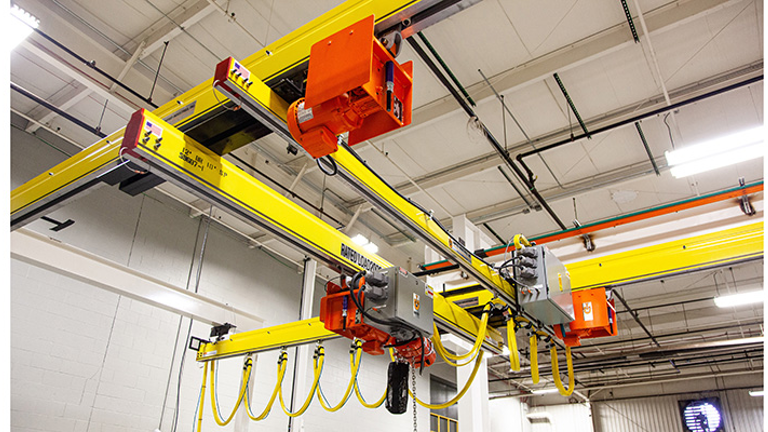
\includegraphics[scale=0.3]{crane.png}
    \caption{\centering{Automated crane. Credit: \href{https://www.materialhandling247.com/product/propath_automated_workstation_crane_by_unified_industries}{Material Handling 247}}}
    
\end{figure}

\item {\bfseries Automated carousels or conveyors:}
Conveyors are AS/R systems that rotate in a loop either horizontally or vertically. A picker is present in a fixed location, whose job is to pick off the items on the conveyor (we can automate the picking system too, as detailed in the next section). However, conveyors are limited to small-sized items. 

\begin{figure}[H]
    
    \centering
    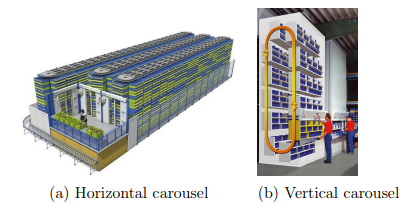
\includegraphics[scale=0.7]{carousel}
    \caption{\centering{Horizontal and vertical automated carousels \cite{main_paper}}}
    
\end{figure}

\item {\bfseries Vertical Lift Module (VLM):}
The function of VLMs is similar to that of carousels, but their operation is different. When an item is required, a VLM's lift-mounted inserter-extractor locates the item and brings it to the picker. This allows the picker to stay in the same location, thereby increasing efficiency. 

\begin{figure}[H]
    
    \centering
    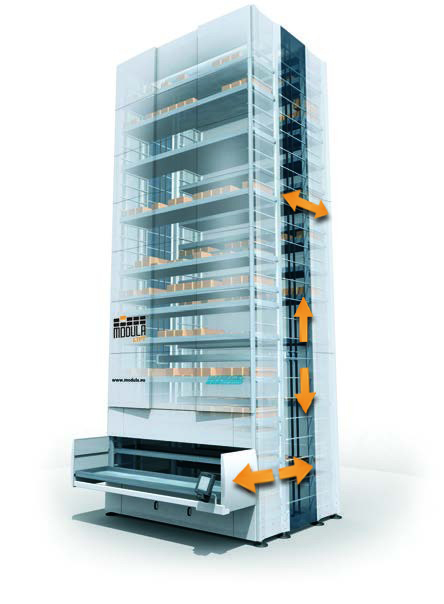
\includegraphics[scale=0.4]{vlm.jpg}
    \caption{\centering{Vertical Lift Module. Credit: \href{https://www.pacificintegrated.com/catalog/storage-and-retrieval-solutions/products/vertical-lift-module-vlm}{Pacific Integrated Handling}}}
    
\end{figure}

\item {\bfseries Shuttles:} Shuttles are automated mobile carts that are used for movement, storage and retrieval of products. A significant advantage of shuttles is that they are highly flexible. The capacity can be increased or decreased based on the number of shuttles used. They also have a high retrieval rate. 

\begin{figure}[H]
    
    \centering
    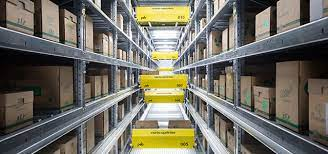
\includegraphics[scale=0.8]{shuttle}
    \caption{\centering{Automated shuttle system. Credit: \href{https://www.psb-gmbh.com/news/automation-in-mid-size-businesses-modular-shuttle-warehouse/}{PSB}}}
    
\end{figure}

\end{itemize}

AIW can employ any (or a combination) of the above automated storage and retrieval systems. They are much more accurate, efficient and time-saving as compared to storage and retrieval manually or by human operated machines.

\subsubsection{Storage}
At the AIW warehouses, the storage is done by employees, with the help of forklifts. Boxes are piled on racks, taking up a lot of space. There is also distance between racks, so that boxes can be retrieved via forklift.

All this space can be utilised much more effectively with the help of automation. The various technologies that may be used are outlined below.
\begin{itemize}
    \item{Multi Deep Compact Storage
\newline\newline
In Multi Deep Compact Storage, AS/R systems are used to store loads double-deep in the racks. This system is extremely useful in places where space minimization is a major concern. The cranes are furnished with double-deep telescopic forks. Deep lane, or compact, multi-deep (3D) AS/R systems can store loads even deeper in storage lanes. 
Generally, in crane-based compact storage system,
\begin{itemize}
    \item {Storage and retrieval (S/R) crane - manages movements in the horizontal and vertical directions of the rack}
\item{Orthogonal conveying mechanism - manages the depth movement\cite{5451644}.}
\end{itemize}}

\begin{figure}[H]
    
    \centering
    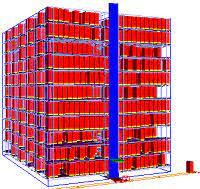
\includegraphics[scale=0.4]{storage.jpg}
    \caption{\centering{Crane-based multi-deep compact storage system \cite{5451644}}}
    
\end{figure}

\item{Chaotic Storage
\newline\newline
The term “chaotic” may sound like something a warehouse must never do. But when it comes to the extremely large size of inventory, this system works. Incoming items are placed randomly on shelves with no regard for specific locations. The most important part of Chaotic storage is inventory or warehouse management software. This software is able to collect information about specific products and their locations by utilising barcodes and barcode scanners. These systems are used to catalogue and track inventory in numerous warehouses. The data held in barcodes is read by a barcode scanner. It is then used to distinguish individual items in multiple warehouses. The exact location and quantity of every item in a warehouse may be found out by scanning the barcode that each pallet or shelf has.}
\end{itemize}

Therefore, depending on the size of the warehouse, either of the above technologies may be used to store items quickly and efficiently.

\subsection{Automated Packaging}

It is typically a warehouse's job to package a shipment before it is delivered to the customer. Packaging protects the item from any damage that could happen during transport or handling. If not done right, a warehouse could incur losses. The AIW warehouses may upgrade their packaging process by utilising the following technologies:
\begin{itemize}
\item{Cartonization

Order volumes are growing, and there is increased demand of faster shipping. Traditionally, warehouses pack all items in standard-size cartons. This is highly inefficient. Very small items, when packed in standard size boxes that are larger, take up space that could have been utilised by another item during shipping. This raises shipping cost and increases shipping time. A solution to this problem is cartonization. Cartonization is a process in which the Warehouse Management System examines each item from an individual order to determine the number and size of each carton required to ship that order. Height, length, width and weight are used as parameters for the cartonization algorithm to figure out the best way to pack individual cartons. Thus, the small items are packed in small cartons, saving cost, reducing shipping time as well as reducing waste.}

\begin{figure}[H]
    
    \centering
    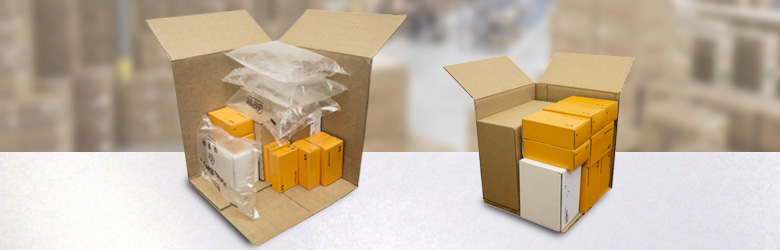
\includegraphics[scale=0.4]{carton.jpg}
    \caption{\centering{Cartonization (Credits: \href{https://www.conveyco.com/technology/automated-packaging/cartonization/}{Conveyco)}}}
    
\end{figure}

\item{Co-bots

Co-bots or collaborative robots work safely alongside human beings. They make the warehouse more efficient by doing repetitive, menial tasks quickly and methodically. After the items are de-palletized and positioned on the conveyer belt, depending on the item, the cobot erects the carton box, loads items in the proper position, and attaches the required labels.}


\item{Automatic packaging machine

As described in Y. Lu et al. \cite{5451644}, the automatic packaging machine has many functions, including bag forming, material filling, sealing temperature control, status display, and fault detection and alarm. The machine controller consists of ATmega128 microcontroller, analog, digital power drive circuit and DC power. On the frontal panel of the intelligent controller, parameter setting is done through the function keys. LCD display shows the parameter setting, running status and fault.
}
\end{itemize}

Thus, by utilising the above mentioned technologies, the AIW warehouses can decrease packaging time, errors, and shipping costs.
\subsection{Automated Product Inspection}

Product inspection is one of the most essential tasks performed in large warehouses like the AIW warehouses. Generally, products with barcodes are inspected using convenient terminals, but there are plenty of products such as bundled items that do not carry a barcode. These items are examined visually by people. This requires a considerable amount of labour and time. Besides this, humans are prone to making errors, which when made during product inspection, could lead to unfavourable outcomes.

The automation technology proposed to solve this problem is that of advanced image recognition.

As outlined in the \href{https://www.nec.com/en/global/techrep/journal/g17/n01/170108.html#:~:text=The%20greatest%20advantage%20of%20the,3}{NEC Technical Journal (Vol.12)}, a distinctive image recognition technology provides immediate information about whether the product to be delivered matches the delivery schedule list. Even in cases where a barcode is not affixed to the item, the actual image of the item may be used to identify it. Advanced image recognition works even when the item is partially hidden or when it is at an oblique angle.

Another useful technology is weight scaling. This enables detection of any excess or deficiency in the weight of the item. This helps in cases where image recognition may fail, such as when the item is obscured or completely hidden.

Visual inspection by humans is also supported. The image of the inspection target item is displayed with the checkpoint name. This allows even workers with little knowledge of the item to perform accurate inspection by contrasting the actual item and the displayed image of the item.

Therefore, a combination of image recognition, weight scaling and visual inspection as a support function may be used to increase efficiency and quality of product inspection at the AIW warehouses.

\begin{figure}[H]
    
    \centering
    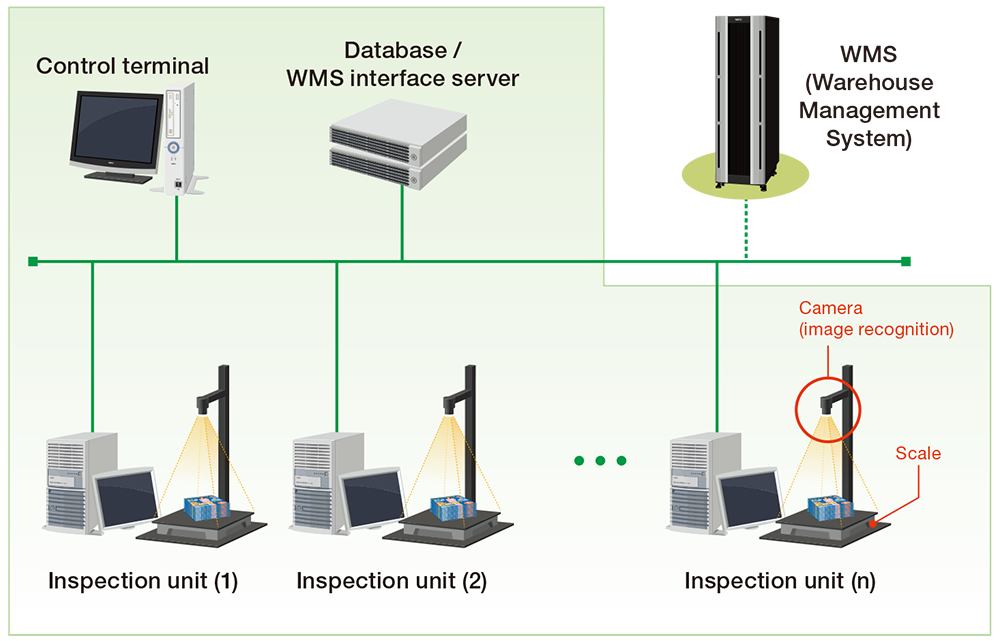
\includegraphics[scale=0.4]{product_ins.png}
    \caption{\centering{Warehouse product inspection system (Credits: \href{https://www.nec.com/en/global/solutions/logistics/kenpin/index.html}{NEC)}}}
    
\end{figure}

\subsection{Automated Product Picking, Loading and Unloading}

In today's world, it is common for orders to be delivered within the following day of placing the order. To achieve this speed, it is important to streamline the process, right from the order being placed to it being delivered, as much as possible. As a part of this effort, it is possible to optimize the product picking process through automation.

Product picking is a warehouse operation where a product is picked from the shelves for the fulfillment of an order. Currently, in AIW, this happens manually. Warehouse workers themselves pick the specific products from the inventory. But, this can be optimized through automation. Below are some methods:

 \begin{figure}[H]
    
    \centering
    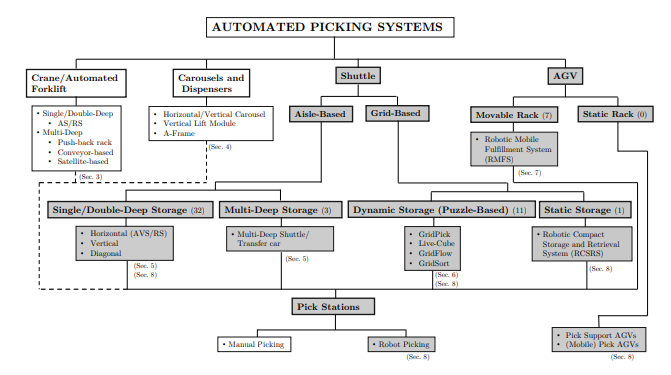
\includegraphics[scale=0.6]{picking.png}
    \caption{\centering{A flowchart of the automated storage, retrieval and picking systems \cite{main_paper}}}
    
    \end{figure}

\begin{itemize}
    \item {\bfseries Automated Guided Vehicles:} 
    Automated Guided Vehicles or AGVs can be used to transport material in warehouses by following a specific marked pathway using radio waves, cameras, magnets or lasers. The guideways for the movement of the AGVs can be made using inductive paths such as metal strips. The data transmission to the control system can be done using infrared or radio waves. Using AGVs can significantly improve picking efficiency.
    
    With an AGV, the picker can add the required items from the shelves into the AGV's roll cage until the roll cage is full. Then, the full AGV is replaced by that with an empty roll cage. The AGV with the filled roll cage automatically transports the items to the depot where it can be loaded and unloaded \cite{main_paper}. 
    
    \begin{figure}[H]
    
    \centering
    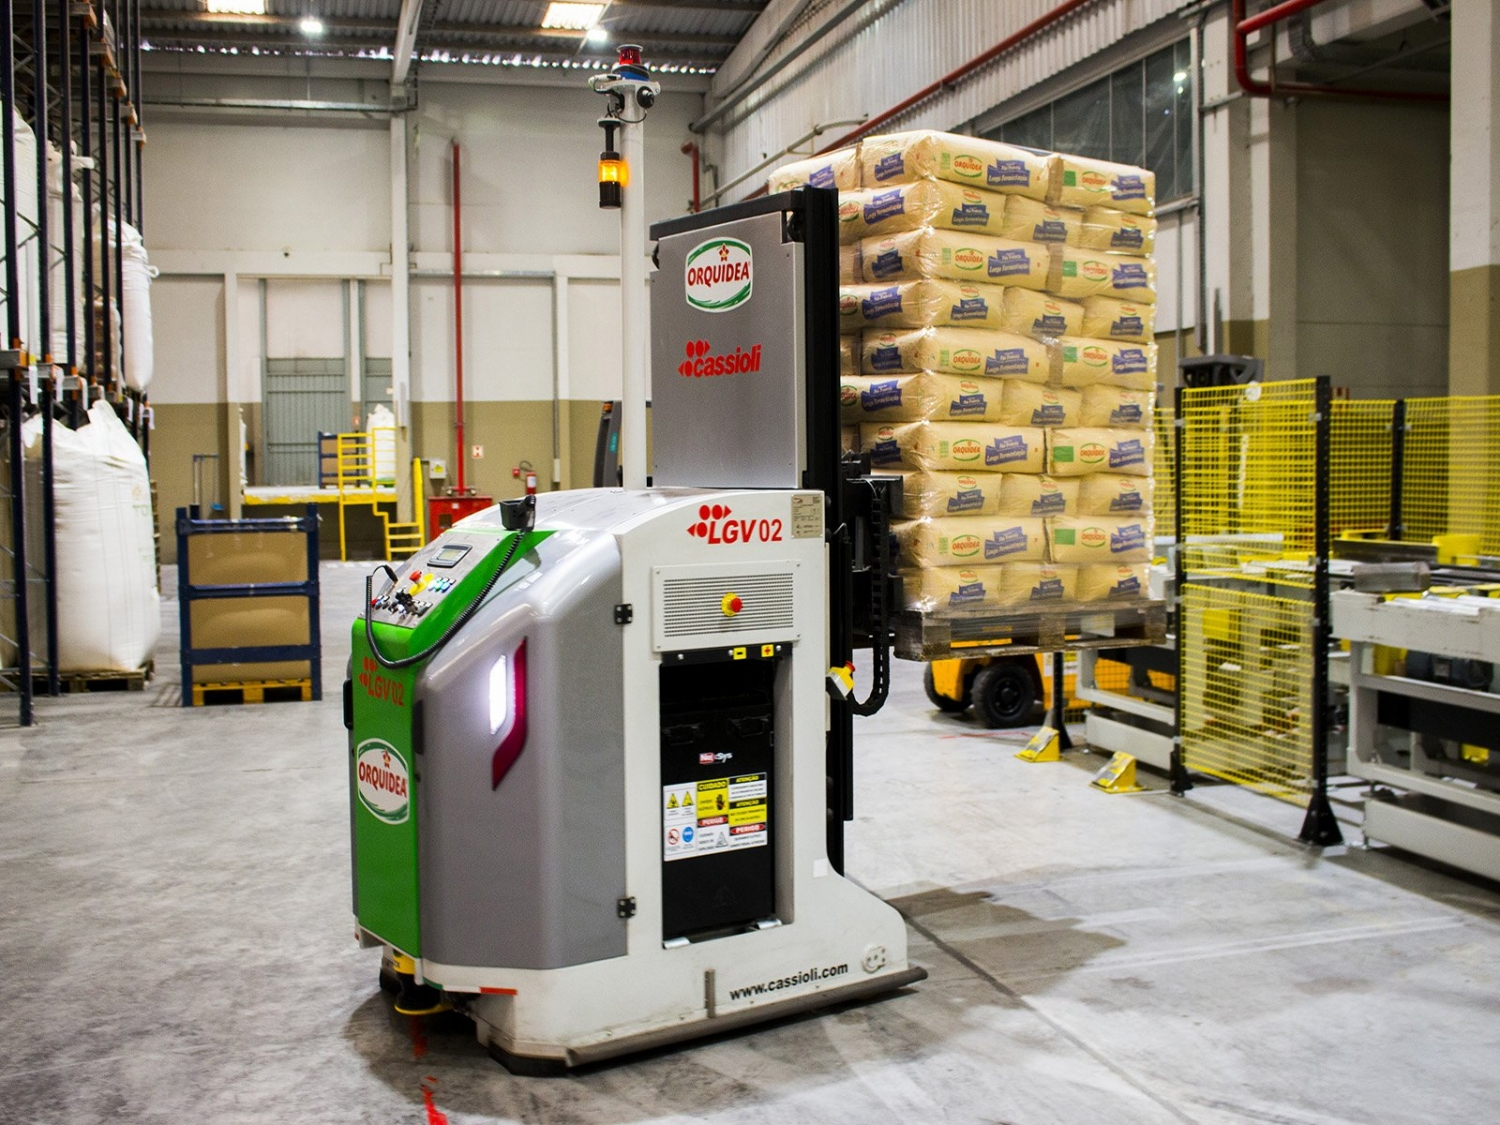
\includegraphics[scale=0.2]{agv.jpg}
    \caption{\centering{An automated guided vehicle. Credits: \href{https://www.cassioli.com/intralogistics-division/automated-vehicles/}{Cassioli Group}}}
    
    \end{figure}
    
    There are also several advanced variants of AGVs. Some AGVs are given all the required items to be picked, and then calculate the most efficient picking route through optimization algorithms. The AGVs take this route so as to minimize the time and redundancy, and allow the picker to follow them. Once all the items have been collected, they return automatically to the required loading/unloading station.
    
    Some other AGVs do not require a human picker at all, but choose the necessary items from the inventory through sophisticated algorithms and specialized robotic arms for the picking.
    
    There are several control functions present in an AGV such as the vehicle control to ensure that the AGV moves along the passive guideways, goal control to guide the vehicle through the layout, blocking control to avoid collisions etc. All of these functions are controlled by a microprocessor. The central control system uses two CPUs: one for the control functions and the other for the communication. Microprocessors such as the 8085 or 8086 can be employed for the control functions.
    
    There are several sensors on the front and rear end of the AGV to ensure that it never moves off the guideway completely. These sensors could be positioning or proximity sensors.
    
    Communication of the AGVs with the central control station can also be carried out by microprocessors such as the Z80, which checks for transmission errors and time-outs \cite{agvmicro}. 
    
    \begin{figure}[H]
    
    \centering
    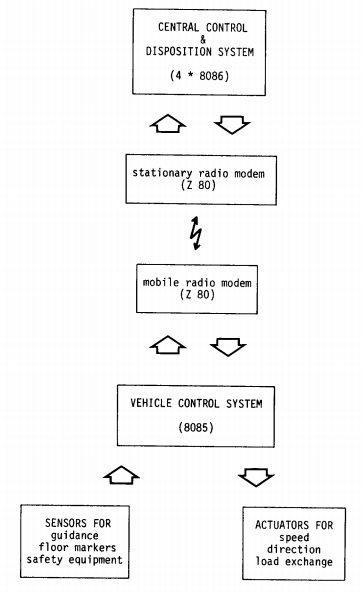
\includegraphics[scale=0.7]{agvmicro.png}
    \caption{\centering{The flowchart represents the control structure of a simple AGV \cite{agvmicro}}}
    
    \end{figure}
    
    \item {\bfseries Robotic Mobile Fulfillment Systems (RMFS)}
    The unique thing about RMFSs is that they bring the products to the picker, instead of letting the picker go to the inventory. By employing such a system, picker productivity doubles \cite{main_paper}.
    
    RMFSs are mobile robots that are able to pick and transport movable shelves and retrieve the detachable shelf racks to the picker for picking the item from the inventory. 
    
    The central control station provides instructions to the robotic drive unit of the RMFS, which picks up the detachable shelf rack (also called the inventory pod) and transports it to the assigned workstation for the human picker.
    
    The advantage of RMFSs is that they are flexible: adding more such mobile robots can improve the efficiency during times of demand.
    
    \begin{figure}[H]
    
    \centering
    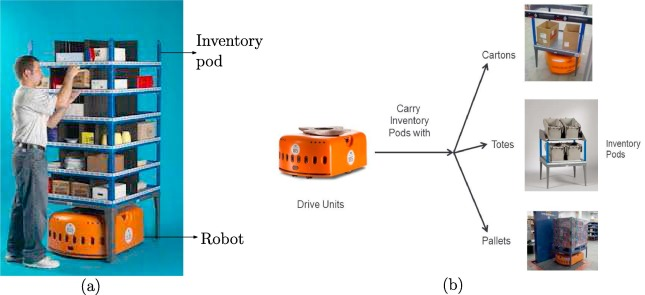
\includegraphics[scale=0.6]{rmfs.jpg}
    \caption{\centering{The Robotic Mobile Fulfillment System moving a detachable shelf rack called an inventory pod \cite{rmfs}}}
    
    \end{figure}
    
    \item {\bfseries Automated Palletization:} 
    In AIW, during the process of picking, loading or unloading, it is typically the worker's job to place the rack of goods onto a pallet for transport. This can be time-consuming and unsafe. Automating this process using a palletizer can reduce the cost of picking, loading and unloading as well as decrease the stress on the warehouse workers.
    
    Modern automated palletizers have a robotic arm (also called an end effector) which can grab the item from a conveyor or a rack and place it onto a pallet. Such automated palletizers have the ability to grab products at high elevation or at ground-level. This is especially useful for AIW as it has ceiling heights ranging from 20-30 feet. 
    
    \begin{figure}[H]
    
    \centering
    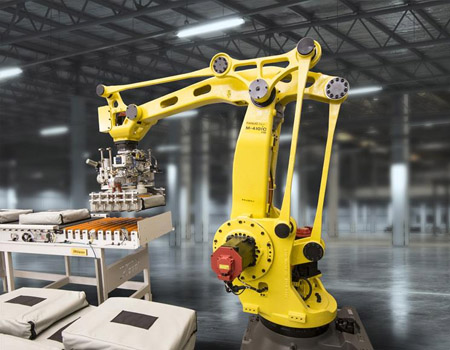
\includegraphics[scale=0.5]{pallet.jpg}
    \caption{\centering{An automated palletizer with a robotic arm. Credit: \href{https://www.jhrobotics.com/palletizing-depalletizing-pg.html}{JH Robotics}}}
    
    \end{figure}
    
\end{itemize}

\subsection{Automated Temperature Control}

AIW also stores food and pharmaceuticals, which require storage in cold temperatures for their preservation. If such perishable goods are not stored at the right temperatures, they may spoil, which results in the warehouse incurring major losses and losing clients. Thus, there is incentive to automate the cold storage system and ensure that the temperature is controlled automatically. 

To adopt an automatic temperature controlled warehouse, {\bfseries battery powered wireless sensors} can be used throughout the facility. Such a system guarantees:

\begin{itemize}
    \item {\bfseries 24/7 Monitoring:} An automated temperature and humidity control system can monitor the temperature conditions round the clock and continuously analyze and record the parameters to check for any unwelcome fluctuations.
    \item {\bfseries Timely Correction:} When the sensors record any unexpected deviations from the ideal conditions, they can alert the warehouse managers immediately so that the necessary corrective actions can be taken. This is especially important as preserving perishable goods can be time sensitive.
    \item {\bfseries Wireless Monitoring:} Adopting wireless sensors throughout the facility ensures that all the necessary information is accessible through a single software. The data processing is also carried out in a timely manner. Certain software can also provide insightful trends of the system.
\end{itemize}

How do such automated temperature sensors function? It is possible to develop such automated tools by programming microcontrollers and creating a partner software application. Temperature sensors record the temperature and humidity information. These sensors then send their observations to a microcontroller, which monitors the temperature and humidity and display the conditions on a monitor. The data can be sent to the warehouse managers through a software application so that they can keep track of the system. 

Common microcontroller used for this application is the AT89S52 which has a high performance while utilizing low power. Temperature sensors such as the SHT10, which measures relative humidity through a capacitive sensor element and a band gap sensor for the temperature measurement. Finally, using a GSM modem such as the TC35i can provide wireless communication to the warehouse managers \cite{Sihombing_2018}.

\bigskip

By developing such automated temperature control systems, AIW can ensure the safety and preservation of perishables and pharmaceuticals.

\subsection{Automated Seasonal or Cyclical Inventory Management}

Some types of products are seasonal in nature: they are primarily in demand only during particular times of the year. For example, raincoats are in demand during the months of June to September, which is the monsoon season in India. Similarly, icecreams, although sold throughout the year, see a distinct spike in demand during the summer months. Some products are more seasonal than others. Regardless of that, it is important to have an efficient seasonal inventory management to reduce wastage, and hence, losses.

When the inventory management is automated, it is possible to access previous years' trends of seasonal products, and thereby forecast the current years' inventory. Using software to assess previous years' inventory information for the seasonal product can help project the current year's information to a fair extent. 

\begin{figure}[H]
    
    \centering
    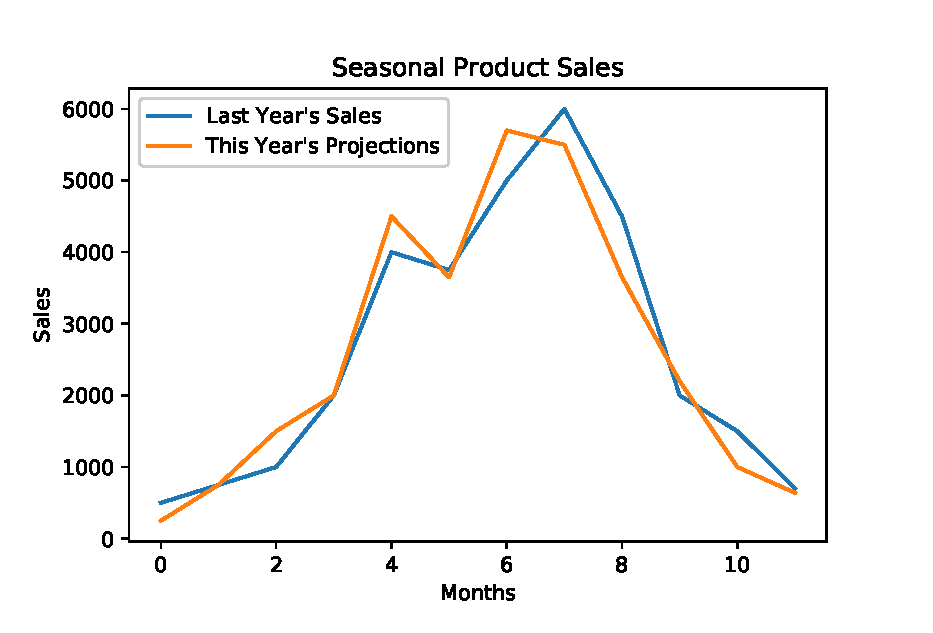
\includegraphics[scale=0.5]{seasonal.eps}
    \caption{\centering{A plot that forecasts the current year's sale of inventory based on the previous season's sales}}
    
\end{figure}

Another method to manage the influx of demand for seasonal products during the on-season is to have dedicated racks, automated storage and retrieval systems and packaging systems for the seasonal products so as to reduce the lead times for such products that incur high demands over a short time.

Using dedicated automated software for controlling the inventory flow and managing the orders of such products also aids in managing seasonal inventory in the warehouse.

\subsection{Automated Security and Monitoring}

For any warehouse, operational and commercial success is contingent on being able to mitigate security risks. Highly valuable stock is stored in warehouses. The most efficient solutions to protect and track items utilise automation. Following are some automation technologies that may be used to upgrade security and monitoring at the AIW warehouses.
\begin{itemize}
    

\item{RFID Location Tracking

Radio-frequency identification (RFID) is a technology solution that makes use of microchips to monitor the locations of items. They transmit information using radio waves, and can be read even if they’re out of sight. They can also recognize a large number of distinct items on a pallet. 

Overall, RFID is a speedy and low-cost method to identify and track merchandise during storage and shipping. It can prevent warehouse theft in a major way.}

\begin{figure}[H]
    
    \centering
    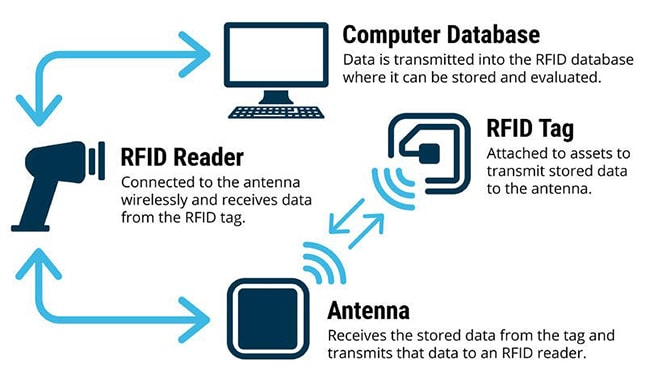
\includegraphics[scale=0.4]{rfid.jpg}
    \caption{\centering{RFID System (Credits: \href{https://comparesoft.com/assets-tracking-software/tracking-business-assets-3-effective-technologies/}{comparesoft.com)}}}
    
\end{figure}

\item{AI security cameras

CCTV is something that has long been used as a security device, and is currently used at the AIW warehouses. But now, there are new IoT (Internet of Things) devices like AI-enabled security cameras available, that can identify faces, track moving targets, and alert warehouse security to potential threats in real time. Now, security guards need not watch multiple areas from a control room. The AI surveillance cameras will provide continuous visibility and threat detection.}

\item{Biometric Systems

Currently, at the AIW warehouses, Automatic Card Access and Door locking systems are provided. However, a much more secure and efficient security solution is a biometric system. Biometrics technology can provide crucial security advantages for warehouses with access checkpoints. These systems scan unique physical characteristics like fingerprints, and thus manage access to warehouse facilities, and prevent unapproved use of machinery.}

\item{Motion detection sensors

Motion detectors sound an alert through the security system’s control panel, when the sensors sense movement. This way, the security system can easily detect when someone is in the warehouse facility when they shouldn’t be.}

\item{Glassbreak detection

A glassbreak detector is a sensor that detects if a panel of glass is broken. Here, a microphone is used to monitor any noise or vibrations coming from the glass, and if the vibrations surpass a specific threshold, the sensor is triggered. This may be useful for large warehouses with glass windows.}

\item{Cyber Security

Another facet of security that is often ignored is cyber security. Devices like AI cameras can be hacked, allowing cybercriminals to gain access to the warehouse network. To prevent this, a secure network needs to be built from the ground up, and utmost priority needs to be given to cyber security.}
\end{itemize}
Therefore, through combining RFID, AI cameras, biometrics, motion detection and glassbreak detection sensors, and giving priority to cyber security, a warehouse can become technologically advanced and more safe and secure than ever before. By implementing the solutions discussed, the security operators at AIW warehouses can increase their efficiency and ability to react to security breaches quickly and effectively. 

\subsection{Automated Fire Systems}

Warehouses are typically very large and store items on very tall shelves. AIW warehouses are no exceptions. There are also more goods and packaging passing through warehouses these days than ever before. Therefore, in warehouses, there is a much higher probability of potential fuel lying around. This translates into a large amount of potential fuel available for an accidental warehouse fire. Due to the same reason, once a warehouse catches fire, it is extremely difficult to put it out.

Currently, the AIW warehouses possess traditional fire alarm and sprinkler systems. These may be upgraded to a more robust and active fire safety system. Some advanced automation technologies that can help with this endeavour are listed below:

\begin{itemize}
    

\item{Video Image Smoke Detection (VISD) technology

The system comprises video-based analytical algorithms that utilise cameras in advanced smoke and flame detection systems. The video is then examined by software that decides if flame or smoke from a fire can be identified. In large warehouses, fires are sometimes difficult to locate. VISD technology solves this problem as well by tracing a fire to its point of origin, thus, resulting in faster extinguishment. VISD is especially useful in large warehouses, where the smoke may never reach a traditional smoke alarm system.}


\item{Integrated Voice Evacuation

Voice evacuation systems are integral to saving lives. They communicate and initiate evacuation procedures in case of an emergency. They are better than fire alarms since fire alarms can be stress and panic-inducing. Voice evacuation technology helps in reducing fear and anxiety. It can be integrated with the security system and programmed accordingly.}

\item{Water mist system

The AIW warehouses are furnished with traditional sprinkler systems. However, they may be replaced by a new and more effective sprinkler technology called the Water Mist suppression systems. In these systems, water is kept under extreme pressure, and released in the form of small droplets or mist. Due to this, the water is able to cover a larger surface area than traditional sprinkler systems. Water mist systems cool the fire while removing oxygen from the seat of the fire. They may be used especially in areas where the items may be damaged if a large quantity of water is sprinkled.

The sprinkler system may also be linked to intelligent devices, so that data can be monitored remotely.}
\end{itemize}

\begin{figure}[H]
    
    \centering
    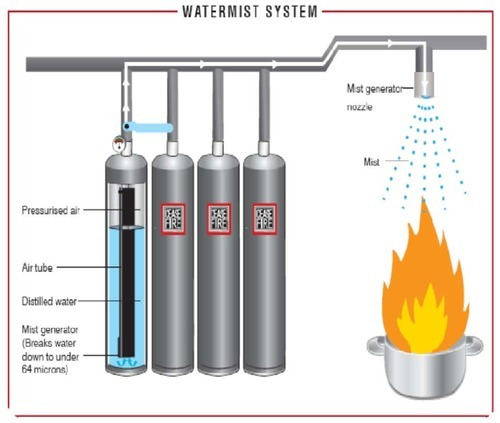
\includegraphics[scale=0.4]{mist.jpg}
    \caption{\centering{Water mist system (Credits: \href{https://www.indiamart.com/proddetail/fire-suppression-with-water-mist-illustration-7673759930.html}{IndiaMART)}}}
    
\end{figure}

Hence, through a combination of VISD technology, Integrated Voice Evacuation and Water mist systems, AIW warehouses may ramp up their fire safety systems with the help of automation.

\subsection{Automated Warehouse Management System}

Currently, AIW uses the software made by its partner company, Storage Solution Pvt Ltd, to maintain database management system to keep track of all the orders and their deliveries. It allows the customers to pick orders online. There is also a paper trail of all the purchases made and the inventory information, as well as the business critical information. These paper records are stored in boxes in the warehouse. 

Maintaining a separate set of paper and digital records about the orders and inventory can become cumbersome. It also becomes more likely for sensitive information to be stolen. To avoid this, all the purchase data can be made electronic and be well protected through a software security system. 

More importantly, the database system of the product orders, tracking, deliveries etc can be combined with the control system of the automated warehousing system \cite{Deng2018DevelopmentOA}. There is a central computer system to control the various automated activities of the warehouse. The warehouse database management system can be combined with this framework to provide an all-in-one software that performs the following functions:

\begin{itemize}
    \item {\bfseries Task Status:}
    This module indicates the current status of the various automation functions that are being undertaken throughout the warehouse.
    \item {\bfseries Warehouse Management:}
    This module describes the inventory information, purchase information and tracking and the customer database.
    \item {\bfseries Business Report:} This module performs statistics on the various product activities and inventory information.
    \item {\bfseries Communication:} This module provides the interface among all the other modules so that the various aspects of the software can work seamlessly.
\end{itemize}

\begin{figure}[H]
    
    \centering
    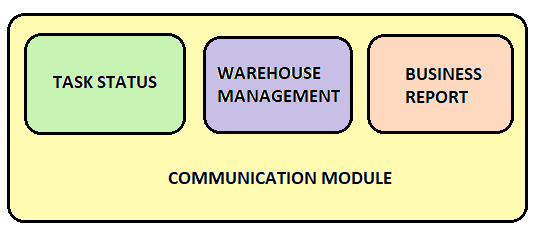
\includegraphics[scale=0.5]{wms}
    \caption{\centering{The various modules used in an automated Warehouse Management System}}
    
\end{figure}

By using such an integrated, automated warehouse management system, AIW can easily access all the required information regarding the warehouse activities in a secure and efficient way without the need for a redundant paper record.



\section{Future Work}

There is vast potential for improving the current system of automated warehouse management. Some examples are:

\begin{itemize}
    \item {\bfseries Product Affinity:}
    Due to the large amount of e-commerce data available presently, it can be used to determine the patterns of customer orders to ensure that products which are often ordered together are stored in close proximity. The more 'affinity' the products have for each other, the relatively closer they are stored.
    
    \item {\bfseries Data Analysis:}
    Analysis of the automated system with respect to certain performance measures such as lead time, throughput etc by integrating all the automation systems together have not been undertaken much. Doing so will provide insight into ways in which the system can be further optimized. 
    
    \item {\bfseries Multi-Line Order Picking:}
    Single-line order picking is where a picker manually picks an item from the inventory to fulfill the order. Multi-line order picking, also know as Batch Order Picking, allows a picker to fulfill several orders at once. This method is much faster and efficient compared to single-line order picking. Batch picking is not as explored in warehouse automation due to its complexity, but there is potential to develop effective methods to perform batch order picking.
    
\end{itemize}

The incorporation of automation in warehouses is not the be-all end-all of logistics. The AIW warehouses must consider how an automated warehouse system would connect holistically with the rest of the systems, for example, the delivery system. Inventory management is also quite important. With the upgradation of technology in the warehouse, the number of items and complexity will likely increase as well. Warehouse space is likely to become a constraint, and in this scenario, inventory management will play an essential role.

Finally, in today's world, automation systems, much like any other domain, is interdisciplinary in nature. Therefore, integrating ideas from other domains can help in the progress of automation systems. For example, operations research continually looks to make a process more efficient through several cutting-edge optimization techniques. Incorporating such research into automation systems, like improving the picking method or the loading/unloading method can reduce the time consumed, thereby increasing productivity. Domains like artificial intelligence can also aid in the improvement of automation systems. Applying sophisticated machine learning algorithms can make us further understand the trends of orders, inventory movement, efficient guideways etc.

\section{Conclusion}

World trade is becoming more and more complex and supply chains are evolving to reflect that. Supply chains are one of the most important elements of today’s globalised economy and the major element of a successful supply chain is logistics. 

For a warehouse, which is an essential part of any logistics operation, keeping up with the ever-changing global trade network is crucial. The only way to do so is through automating and adopting advanced technologies.

 The AIW mission is to provide cost-efficient and high quality warehouse distribution with value-added services. This mission can be realised by automating the facilities. In a complex warehouse system, such as the AIW warehouses, the move to a highly automated model can be intimidating, but failing to change and adapt will have far worse consequences.

Knowing that automation is the key to modern warehousing, we attempted, in this report, to transform AIW warehouses into technologically-advanced warehouses and solve some of the problems that they may face with the help of technology. 

\printbibliography

\end{document}
